\begin{comment}
\chapter{Amortized analysis}

\index{amortized analysis}

The time complexity of an algorithm
is often easy to analyze
just by examining the structure
of the algorithm:
what loops does the algorithm contain
and how many times the loops are performed.
However, sometimes a straightforward analysis
does not give a true picture of the efficiency of the algorithm.

\key{Amortized analysis} can be used to analyze
algorithms that contain operations whose
time complexity varies.
The idea is to estimate the total time used to
all such operations during the
execution of the algorithm, instead of focusing
on individual operations.
\end{comment}

\chapter{ならし解析}

\index{amortized analysis}
\index{ならし解析}

アルゴリズムの時間計算量は、しばしば
アルゴリズムの構造から簡単に計算できる:
例えばアルゴリズムがいくつのループを含み、各ループが
何回ループするかを数えればよい。
しかし、しばしばそのような単純な分析では十分にアルゴリズムの
真の姿をあぶりだせないことがある。

ならし解析(償却解析、\key{amortized analysis})は時間計算量が変化するような
演算を含むアルゴリズムを分析するのに利用できる。
基本となるアイデアは、個々の処理に注目するのではなく、
アルゴリズム実行の全体で各処理がどのように実行されるかから
実行時間を推測することである。

\begin{comment}
\section{Two pointers method}

\index{two pointers method}

In the \key{two pointers method},
two pointers are used to
iterate through the array values.
Both pointers can move to one direction only,
which ensures that the algorithm works efficiently.
Next we discuss two problems that can be solved
using the two pointers method.
\end{comment}

\section{尺取り法}

\index{two pointers method}
\index{尺取り法}

尺取り法(\key{two pointers method})では、
配列全体を辿るのに2つのポインタを使う。
両ポインタは一方向のみ動かすことで、アルゴリズムが
効率的に動作することを保証する。
ここから、尺取り法で解ける2つの問題について論じていこう。

\begin{comment}
\subsubsection{Subarray sum}

As the first example,
consider a problem where we are
given an array of $n$ positive integers
and a target sum $x$,
and we want to find a subarray whose sum is $x$
or report that there is no such subarray.

For example, the array
\end{comment}

\subsubsection{部分列の総和}

最初の例は、$n$要素の正整数の配列と求めるべき総和$x$が与えられたとき、
和が$x$となる部分列を探す問題である。

例えば、配列
\begin{center}
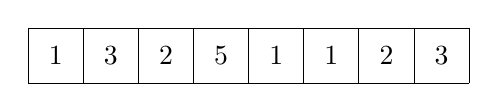
\begin{tikzpicture}[scale=0.7]
\draw (0,0) grid (8,1);

\node at (0.5,0.5) {$1$};
\node at (1.5,0.5) {$3$};
\node at (2.5,0.5) {$2$};
\node at (3.5,0.5) {$5$};
\node at (4.5,0.5) {$1$};
\node at (5.5,0.5) {$1$};
\node at (6.5,0.5) {$2$};
\node at (7.5,0.5) {$3$};
\end{tikzpicture}
\end{center}
\begin{comment}
\end{comment}
は和が8となる部分列を含む。
\begin{center}
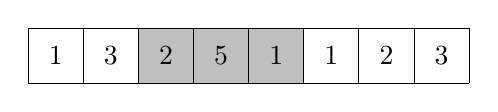
\begin{tikzpicture}[scale=0.7]
\fill[color=lightgray] (2,0) rectangle (5,1);
\draw (0,0) grid (8,1);

\node at (0.5,0.5) {$1$};
\node at (1.5,0.5) {$3$};
\node at (2.5,0.5) {$2$};
\node at (3.5,0.5) {$5$};
\node at (4.5,0.5) {$1$};
\node at (5.5,0.5) {$1$};
\node at (6.5,0.5) {$2$};
\node at (7.5,0.5) {$3$};
\end{tikzpicture}
\end{center}

\begin{comment}
This problem can be solved in
$O(n)$ time by using the two pointers method.
The idea is to maintain pointers that point to the
first and last value of a subarray.
On each turn, the left pointer moves one step
to the right, and the right pointer moves to the right
as long as the resulting subarray sum is at most $x$.
If the sum becomes exactly $x$,
a solution has been found.

As an example, consider the following array
and a target sum $x=8$:
\end{comment}

この問題は尺取り法で$O(n)$時間で解くことができる。
そのためのアイデアは、部分列の先頭と末尾のポインタを管理していくことである。
処理1ループごとに、先頭のポインタを1つ後ろに動かし、
その際末尾のポインタを部分列の総和が$x$以下である限りできるだけ動かすことにする。
もし途中で和がぴったり$x$になったら、解が見つかったことになる。

以下の例では、次の配列と求める総和$x=8$の場合を示す:
\begin{center}
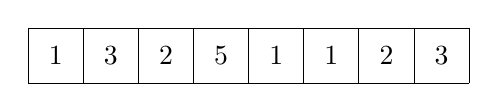
\begin{tikzpicture}[scale=0.7]
\draw (0,0) grid (8,1);

\node at (0.5,0.5) {$1$};
\node at (1.5,0.5) {$3$};
\node at (2.5,0.5) {$2$};
\node at (3.5,0.5) {$5$};
\node at (4.5,0.5) {$1$};
\node at (5.5,0.5) {$1$};
\node at (6.5,0.5) {$2$};
\node at (7.5,0.5) {$3$};
\end{tikzpicture}
\end{center}

\begin{comment}
The initial subarray contains the values
1, 3 and 2 whose sum is 6:
\end{comment}

最初の部分列は、値1,3,2を含み、その和は6である。
\begin{center}
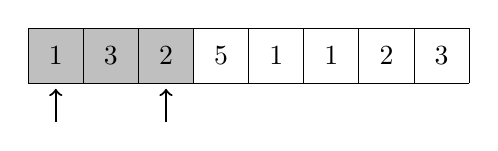
\begin{tikzpicture}[scale=0.7]
\fill[color=lightgray] (0,0) rectangle (3,1);
\draw (0,0) grid (8,1);

\node at (0.5,0.5) {$1$};
\node at (1.5,0.5) {$3$};
\node at (2.5,0.5) {$2$};
\node at (3.5,0.5) {$5$};
\node at (4.5,0.5) {$1$};
\node at (5.5,0.5) {$1$};
\node at (6.5,0.5) {$2$};
\node at (7.5,0.5) {$3$};

\draw[thick,->] (0.5,-0.7) -- (0.5,-0.1);
\draw[thick,->] (2.5,-0.7) -- (2.5,-0.1);
\end{tikzpicture}
\end{center}

\begin{comment}
Then, the left pointer moves one step to the right.
The right pointer does not move, because otherwise
the subarray sum would exceed $x$.
\end{comment}

次に、先頭のポインタを1つ右に動かす。
末尾のポインタは、これ以上動かすと和が$x$を超えてしまうため
動かさない。

\begin{center}
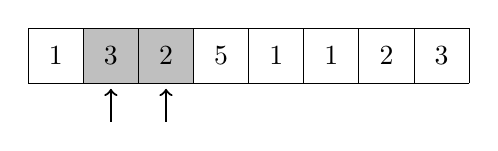
\begin{tikzpicture}[scale=0.7]
\fill[color=lightgray] (1,0) rectangle (3,1);
\draw (0,0) grid (8,1);

\node at (0.5,0.5) {$1$};
\node at (1.5,0.5) {$3$};
\node at (2.5,0.5) {$2$};
\node at (3.5,0.5) {$5$};
\node at (4.5,0.5) {$1$};
\node at (5.5,0.5) {$1$};
\node at (6.5,0.5) {$2$};
\node at (7.5,0.5) {$3$};

\draw[thick,->] (1.5,-0.7) -- (1.5,-0.1);
\draw[thick,->] (2.5,-0.7) -- (2.5,-0.1);
\end{tikzpicture}
\end{center}

\begin{comment}
Again, the left pointer moves one step to the right,
and this time the right pointer moves three
steps to the right.
The subarray sum is $2+5+1=8$, so a subarray
whose sum is $x$ has been found.
\end{comment}

再度先頭のポインタを右に動かし、
今度は右のポインタを2つ右に動かす。
そうすると得られる部分列の和は$2+5+1=8$となり、
求める部分列を見つけることができた。

\begin{center}
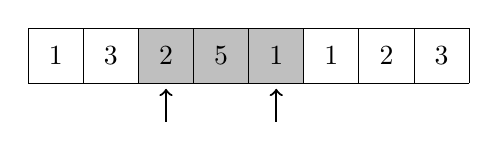
\begin{tikzpicture}[scale=0.7]
\fill[color=lightgray] (2,0) rectangle (5,1);
\draw (0,0) grid (8,1);

\node at (0.5,0.5) {$1$};
\node at (1.5,0.5) {$3$};
\node at (2.5,0.5) {$2$};
\node at (3.5,0.5) {$5$};
\node at (4.5,0.5) {$1$};
\node at (5.5,0.5) {$1$};
\node at (6.5,0.5) {$2$};
\node at (7.5,0.5) {$3$};

\draw[thick,->] (2.5,-0.7) -- (2.5,-0.1);
\draw[thick,->] (4.5,-0.7) -- (4.5,-0.1);
\end{tikzpicture}
\end{center}

\begin{comment}
The running time of the algorithm depends on
the number of steps the right pointer moves.
While there is no useful upper bound on how many steps the
pointer can move on a \emph{single} turn.
we know that the pointer moves \emph{a total of}
$O(n)$ steps during the algorithm,
because it only moves to the right.

Since both the left and right pointer
move $O(n)$ steps during the algorithm,
the algorithm works in $O(n)$ time.
\end{comment}

このアルゴリズムの実行時間は末尾のポインタの移動回数に
依存する。
先頭ポインタを\emph{1回}動かす間に末尾のポインタを
何回動かすことになるかはわからないが、
\emph{合計で}$O(n)$回程度になることはわかる。
末尾のポインタは配列を一方向にしか動けないためである。

結局、先頭も末尾も両ポインタは$O(n)$回動くので、
このアルゴリズムは全体で$O(n)$時間で動作する。

\begin{comment}
\subsubsection{2SUM problem}

\index{2SUM problem}

Another problem that can be solved using
the two pointers method is the following problem,
also known as the \key{2SUM problem}:
given an array of $n$ numbers and
a target sum $x$, find
two array values such that their sum is $x$,
or report that no such values exist.

To solve the problem, we first
sort the array values in increasing order.
After that, we iterate through the array using
two pointers.
The left pointer starts at the first value
and moves one step to the right on each turn.
The right pointer begins at the last value
and always moves to the left until the sum of the
left and right value is at most $x$.
If the sum is exactly $x$,
a solution has been found.

For example, consider the following array
and a target sum $x=12$:
\end{comment}

\subsubsection{2サム問題}

\index{2SUM problem}
\index{2サム問題}

尺取り法で解ける別の問題の例には2サム問題(\key{2SUM problem})がある。
長さ$n$の配列と目標の和$x$が与えられたとき、
和が$x$となる2要素を探す問題である。

解法としては、まず数列を昇順ソートしよう。
その後、2つのポインタで配列を探索していく。
左のポインタは先頭から末尾に1つずつ移動していく。
右のポインタは逆に末尾から先頭に向けて移動していく。
その際、両ポインタの指す要素の和が$x$以下となるように移動する。
もし和がちょうど$x$になるなら、求める解を見つけたことになる。

以下の配列について、目標の和を$x=12$とした場合の例を考える:

\begin{center}
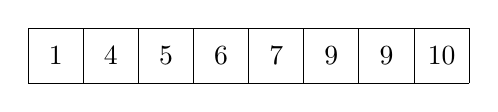
\begin{tikzpicture}[scale=0.7]
\draw (0,0) grid (8,1);

\node at (0.5,0.5) {$1$};
\node at (1.5,0.5) {$4$};
\node at (2.5,0.5) {$5$};
\node at (3.5,0.5) {$6$};
\node at (4.5,0.5) {$7$};
\node at (5.5,0.5) {$9$};
\node at (6.5,0.5) {$9$};
\node at (7.5,0.5) {$10$};
\end{tikzpicture}
\end{center}

\begin{comment}
The initial positions of the pointers
are as follows.
The sum of the values is $1+10=11$
that is smaller than $x$.
\end{comment}

初期状態で両ポインタの位置は下記のようになる。
両者の指す要素の和は$1+10=11$であり
$x$より小さい。

\begin{center}
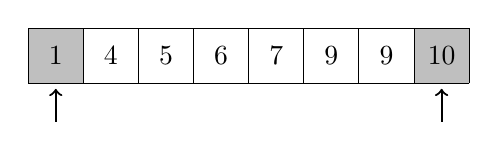
\begin{tikzpicture}[scale=0.7]
\fill[color=lightgray] (0,0) rectangle (1,1);
\fill[color=lightgray] (7,0) rectangle (8,1);
\draw (0,0) grid (8,1);

\node at (0.5,0.5) {$1$};
\node at (1.5,0.5) {$4$};
\node at (2.5,0.5) {$5$};
\node at (3.5,0.5) {$6$};
\node at (4.5,0.5) {$7$};
\node at (5.5,0.5) {$9$};
\node at (6.5,0.5) {$9$};
\node at (7.5,0.5) {$10$};

\draw[thick,->] (0.5,-0.7) -- (0.5,-0.1);
\draw[thick,->] (7.5,-0.7) -- (7.5,-0.1);
\end{tikzpicture}
\end{center}

\begin{comment}
Then the left pointer moves one step to the right.
The right pointer moves three steps to the left,
and the sum becomes $4+7=11$.
\end{comment}

左のポインタを1つ右に動かす。
右のポインタは対応して3つ左に動かすと、
和は$4+7=11$となる。

\begin{center}
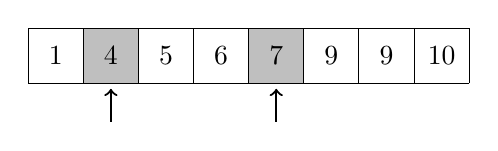
\begin{tikzpicture}[scale=0.7]
\fill[color=lightgray] (1,0) rectangle (2,1);
\fill[color=lightgray] (4,0) rectangle (5,1);
\draw (0,0) grid (8,1);

\node at (0.5,0.5) {$1$};
\node at (1.5,0.5) {$4$};
\node at (2.5,0.5) {$5$};
\node at (3.5,0.5) {$6$};
\node at (4.5,0.5) {$7$};
\node at (5.5,0.5) {$9$};
\node at (6.5,0.5) {$9$};
\node at (7.5,0.5) {$10$};

\draw[thick,->] (1.5,-0.7) -- (1.5,-0.1);
\draw[thick,->] (4.5,-0.7) -- (4.5,-0.1);
\end{tikzpicture}
\end{center}

\begin{comment}
After this, the left pointer moves one step to the right again.
The right pointer does not move, and a solution
$5+7=12$ has been found.
\end{comment}

その後、左のポインタをもう一つ右に動かす。
この場合右のポインタはこれ以上動かず、解として$5+7=12$を得られる。

\begin{center}
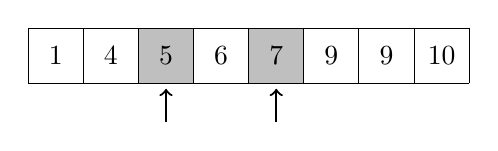
\begin{tikzpicture}[scale=0.7]
\fill[color=lightgray] (2,0) rectangle (3,1);
\fill[color=lightgray] (4,0) rectangle (5,1);
\draw (0,0) grid (8,1);

\node at (0.5,0.5) {$1$};
\node at (1.5,0.5) {$4$};
\node at (2.5,0.5) {$5$};
\node at (3.5,0.5) {$6$};
\node at (4.5,0.5) {$7$};
\node at (5.5,0.5) {$9$};
\node at (6.5,0.5) {$9$};
\node at (7.5,0.5) {$10$};

\draw[thick,->] (2.5,-0.7) -- (2.5,-0.1);
\draw[thick,->] (4.5,-0.7) -- (4.5,-0.1);
\end{tikzpicture}
\end{center}

\begin{comment}
The running time of the algorithm is
$O(n \log n)$, because it first sorts
the array in $O(n \log n)$ time,
and then both pointers move $O(n)$ steps.

Note that it is possible to solve the problem
in another way in $O(n \log n)$ time using binary search.
In such a solution, we iterate through the array
and for each array value, we try to find another
value that yields the sum $x$.
This can be done by performing $n$ binary searches,
each of which takes $O(\log n)$ time.
\end{comment}

このアルゴリズムの実行時間は$O(n \log n)$である。
というのも、尺取り法部分は$O(n)$回のステップで処理が完了するが、
最初のソートに$O(n \log n)$時間かかるためである。

なお、この問題は二分探索を使い$O(n \log n)$時間で解く別解もある。
各要素について、それと対にして和が$x$となる要素を探す解法である。
二分探索を使って探すようにすると、$n$回二分探索をするので
全体で$O(\log n)$の時間がかかる。

\begin{comment}
\index{3SUM problem}
A more difficult problem is 
the \key{3SUM problem} that asks to
find \emph{three} array values
whose sum is $x$.
Using the idea of the above algorithm,
this problem can be solved in $O(n^2)$ time\footnote{For a long time,
it was thought that solving
the 3SUM problem more efficiently than in $O(n^2)$ time
would not be possible.
However, in 2014, it turned out \cite{gro14}
that this is not the case.}.
Can you see how?
\end{comment}

\index{3SUM problem}
\index{3サム問題}

より難しい問題として、\emph{3つの}要素の和が$x$となる
要素を求める\key{3サム問題がある}。
これは先ほどのアイデアを応用すると、$O(n^2)$時間で解くことができる。
\footnote{長い間、この問題は$O(n^2)$時間より短くは解けないと思われていた。
しかし、2014年そうでないことが分かった。\cite{gro14}}
どのようにすればよいかわかるだろうか?

\begin{comment}
\section{Nearest smaller elements}

\index{nearest smaller elements}

Amortized analysis is often used to
estimate the number of operations
performed on a data structure.
The operations may be distributed unevenly so
that most operations occur during a
certain phase of the algorithm, but the total
number of the operations is limited.

As an example, consider the problem
of finding for each array element
the \key{nearest smaller element}, i.e.,
the first smaller element that precedes the element
in the array.
It is possible that no such element exists,
in which case the algorithm should report this.
Next we will see how the problem can be
efficiently solved using a stack structure.
\end{comment}

\section{nearest smaller elements}

\index{nearest smaller elements}

ならし解析はしばしばデータ構造に対する処理数を概算するのにも用いる。
アルゴリズムの個々のフェーズで実施する処理回数が不均等でも、
全体で実施する処理量の上界が求められることはしばしばある。

例として、数値の配列が与えられたとき、\key{nearest smaller element} \footnote{
訳注:いい和訳が見つかりませんでした。}を求めることを考える。
これは、数列の各要素に対し、その手前の中で最も近くにある
自身より小さい値を持つ要素のことである。
(そのような要素が存在しない場合もある。)
次に、スタックを使いこの問題を効率的に解く様子を見ていこう。

\begin{comment}
We go through the array from left to right
and maintain a stack of array elements.
At each array position, we remove elements from the stack
until the top element is smaller than the
current element, or the stack is empty.
Then, we report that the top element is
the nearest smaller element of the current element,
or if the stack is empty, there is no such element.
Finally, we add the current element to the stack.

As an example, consider the following array:
\end{comment}

配列を左から右に辿っていき、同時に配列要素からなるスタックを管理して以降。
配列の各位置において、スタックの最上位が自身の値より小さいか空になるまで
最上位をpopすることを繰り返していこう。
そうすると、スタックに残った最上位の値が現在の要素に最も近いより小さい値となる。
その後、自身をスタックに積む。

例えば以下の配列を考えよう:
\begin{center}
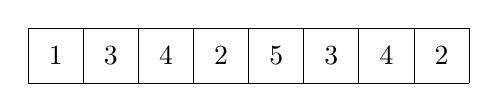
\begin{tikzpicture}[scale=0.7]
\draw (0,0) grid (8,1);

\node at (0.5,0.5) {$1$};
\node at (1.5,0.5) {$3$};
\node at (2.5,0.5) {$4$};
\node at (3.5,0.5) {$2$};
\node at (4.5,0.5) {$5$};
\node at (5.5,0.5) {$3$};
\node at (6.5,0.5) {$4$};
\node at (7.5,0.5) {$2$};
\end{tikzpicture}
\end{center}

\begin{comment}
First, the elements 1, 3 and 4 are added to the stack,
because each element is larger than the previous element.
Thus, the nearest smaller element of 4 is 3,
and the nearest smaller element of 3 is 1.
\end{comment}

最初、要素1,3,4はこの順でスタックに積まれる。
というのも、各要素は直前の値より大きいためである。
その結果、4に最も近いより小さい値は3であり、
3に最も近いより小さい値は1となる。
\begin{center}
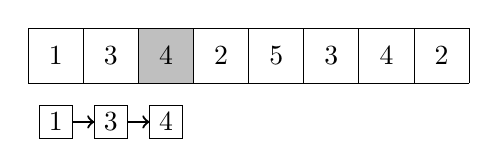
\begin{tikzpicture}[scale=0.7]
\fill[color=lightgray] (2,0) rectangle (3,1);
\draw (0,0) grid (8,1);

\node at (0.5,0.5) {$1$};
\node at (1.5,0.5) {$3$};
\node at (2.5,0.5) {$4$};
\node at (3.5,0.5) {$2$};
\node at (4.5,0.5) {$5$};
\node at (5.5,0.5) {$3$};
\node at (6.5,0.5) {$4$};
\node at (7.5,0.5) {$2$};

\draw (0.2,0.2-1.2) rectangle (0.8,0.8-1.2);
\draw (1.2,0.2-1.2) rectangle (1.8,0.8-1.2);
\draw (2.2,0.2-1.2) rectangle (2.8,0.8-1.2);

\node at (0.5,0.5-1.2) {$1$};
\node at (1.5,0.5-1.2) {$3$};
\node at (2.5,0.5-1.2) {$4$};

\draw[->,thick] (0.8,0.5-1.2) -- (1.2,0.5-1.2);
\draw[->,thick] (1.8,0.5-1.2) -- (2.2,0.5-1.2);
\end{tikzpicture}
\end{center}

\begin{comment}
The next element 2 is smaller than the two top
elements in the stack.
Thus, the elements 3 and 4 are removed from the stack,
and then the element 2 is added to the stack.
Its nearest smaller element is 1:
\end{comment}

次の要素2は、スタックの上位2要素より小さい。
そのため3,4はスタックから取り除かれ、2がスタックに積まれる。
よって2に最も近いより小さい値は1である:
\begin{center}
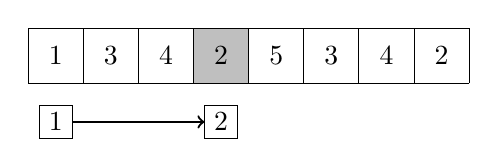
\begin{tikzpicture}[scale=0.7]
\fill[color=lightgray] (3,0) rectangle (4,1);
\draw (0,0) grid (8,1);

\node at (0.5,0.5) {$1$};
\node at (1.5,0.5) {$3$};
\node at (2.5,0.5) {$4$};
\node at (3.5,0.5) {$2$};
\node at (4.5,0.5) {$5$};
\node at (5.5,0.5) {$3$};
\node at (6.5,0.5) {$4$};
\node at (7.5,0.5) {$2$};

\draw (0.2,0.2-1.2) rectangle (0.8,0.8-1.2);
\draw (3.2,0.2-1.2) rectangle (3.8,0.8-1.2);

\node at (0.5,0.5-1.2) {$1$};
\node at (3.5,0.5-1.2) {$2$};

\draw[->,thick] (0.8,0.5-1.2) -- (3.2,0.5-1.2);
\end{tikzpicture}
\end{center}

\begin{comment}
Then, the element 5 is larger than the element 2,
so it will be added to the stack, and
its nearest smaller element is 2:
\end{comment}

次の要素5は、スタックの最上位である2より大きい。
そのため5がスタックに積まれる。
5に最も近いより小さい値は2となる:
\begin{center}
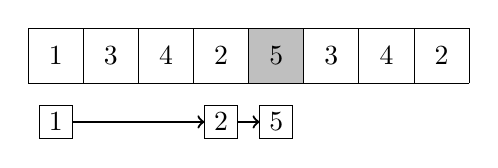
\begin{tikzpicture}[scale=0.7]
\fill[color=lightgray] (4,0) rectangle (5,1);
\draw (0,0) grid (8,1);

\node at (0.5,0.5) {$1$};
\node at (1.5,0.5) {$3$};
\node at (2.5,0.5) {$4$};
\node at (3.5,0.5) {$2$};
\node at (4.5,0.5) {$5$};
\node at (5.5,0.5) {$3$};
\node at (6.5,0.5) {$4$};
\node at (7.5,0.5) {$2$};

\draw (0.2,0.2-1.2) rectangle (0.8,0.8-1.2);
\draw (3.2,0.2-1.2) rectangle (3.8,0.8-1.2);
\draw (4.2,0.2-1.2) rectangle (4.8,0.8-1.2);

\node at (0.5,0.5-1.2) {$1$};
\node at (3.5,0.5-1.2) {$2$};
\node at (4.5,0.5-1.2) {$5$};

\draw[->,thick] (0.8,0.5-1.2) -- (3.2,0.5-1.2);
\draw[->,thick] (3.8,0.5-1.2) -- (4.2,0.5-1.2);
\end{tikzpicture}
\end{center}

\begin{comment}
After this, the element 5 is removed from the stack
and the elements 3 and 4 are added to the stack:
\end{comment}

その後、5は取り除かれ3,4がスタックに積まれる:
\begin{center}
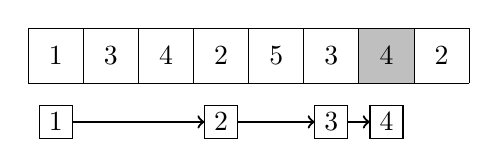
\begin{tikzpicture}[scale=0.7]
\fill[color=lightgray] (6,0) rectangle (7,1);
\draw (0,0) grid (8,1);

\node at (0.5,0.5) {$1$};
\node at (1.5,0.5) {$3$};
\node at (2.5,0.5) {$4$};
\node at (3.5,0.5) {$2$};
\node at (4.5,0.5) {$5$};
\node at (5.5,0.5) {$3$};
\node at (6.5,0.5) {$4$};
\node at (7.5,0.5) {$2$};

\draw (0.2,0.2-1.2) rectangle (0.8,0.8-1.2);
\draw (3.2,0.2-1.2) rectangle (3.8,0.8-1.2);
\draw (5.2,0.2-1.2) rectangle (5.8,0.8-1.2);
\draw (6.2,0.2-1.2) rectangle (6.8,0.8-1.2);

\node at (0.5,0.5-1.2) {$1$};
\node at (3.5,0.5-1.2) {$2$};
\node at (5.5,0.5-1.2) {$3$};
\node at (6.5,0.5-1.2) {$4$};

\draw[->,thick] (0.8,0.5-1.2) -- (3.2,0.5-1.2);
\draw[->,thick] (3.8,0.5-1.2) -- (5.2,0.5-1.2);
\draw[->,thick] (5.8,0.5-1.2) -- (6.2,0.5-1.2);
\end{tikzpicture}
\end{center}

\begin{comment}
Finally, all elements except 1 are removed
from the stack and the last element 2
is added to the stack:
\end{comment}

最終的に1以外の要素は取り除かれ、
最後の2がスタックに積まれる:

\begin{center}
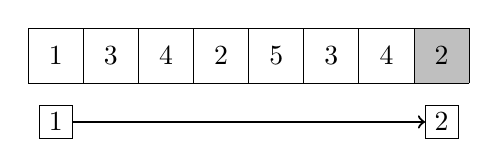
\begin{tikzpicture}[scale=0.7]
\fill[color=lightgray] (7,0) rectangle (8,1);
\draw (0,0) grid (8,1);

\node at (0.5,0.5) {$1$};
\node at (1.5,0.5) {$3$};
\node at (2.5,0.5) {$4$};
\node at (3.5,0.5) {$2$};
\node at (4.5,0.5) {$5$};
\node at (5.5,0.5) {$3$};
\node at (6.5,0.5) {$4$};
\node at (7.5,0.5) {$2$};

\draw (0.2,0.2-1.2) rectangle (0.8,0.8-1.2);
\draw (7.2,0.2-1.2) rectangle (7.8,0.8-1.2);

\node at (0.5,0.5-1.2) {$1$};
\node at (7.5,0.5-1.2) {$2$};

\draw[->,thick] (0.8,0.5-1.2) -- (7.2,0.5-1.2);
\end{tikzpicture}
\end{center}

\begin{comment}
The efficiency of the algorithm depends on
the total number of stack operations.
If the current element is larger than
the top element in the stack, it is directly
added to the stack, which is efficient.
However, sometimes the stack can contain several
larger elements and it takes time to remove them.
Still, each element is added \emph{exactly once} to the stack
and removed \emph{at most once} from the stack.
Thus, each element causes $O(1)$ stack operations,
and the algorithm works in $O(n)$ time.
\end{comment}

このアルゴリズムの効率は、スタックに対する処理の総回数による、
もし現在の要素がスタックの最上位より大きければ、単に
要素を最上位に積むだけでよく、効率的である。
しかし、しばしばスタックに自身より大きな要素が積まれており、
それらを取り除くのに時間がかかる場合がある。
しかし、各要素は\emph{必ず1回だけ}スタックに積まれ、\emph{必ず1回だけ}
スタックから取り除かれる。
よって各要素のスタック処理回数は$O(1)$回であり、
アルゴリズムは$O(N)$時間で動作する。

\begin{comment}
\section{Sliding window minimum}

\index{sliding window}
\index{sliding window minimum}

A \key{sliding window} is a constant-size subarray
that moves from left to right through the array.
At each window position,
we want to calculate some information
about the elements inside the window.
In this section, we focus on the problem
of maintaining the \key{sliding window minimum},
which means that
we should report the smallest value inside each window.
\end{comment}

\section{スライド最小値}

\index{sliding window}
\index{sliding window minimum}
\index{スライド最小値}

スライドウインドウ(\key{sliding window})は
配列中を左から右に移動する固定サイズの部分列である。
このウインドウの位置ごとに、ウインドウ内の要素に関し何らかの情報を計算したいとする。
この章では、スライド最小値(\key{sliding window minimum})に焦点を当てる。
これはウインドウ内の最小値を求めるものである。

\begin{comment}
The sliding window minimum can be calculated
using a similar idea that we used to calculate
the nearest smaller elements.
We maintain a queue
where each element is larger than
the previous element,
and the first element
always corresponds to the minimum element inside the window.
After each window move,
we remove elements from the end of the queue
until the last queue element
is smaller than the new window element,
or the queue becomes empty.
We also remove the first queue element
if it is not inside the window anymore.
Finally, we add the new window element
to the end of the queue.

As an example, consider the following array:
\end{comment}

スライド最小値は、先ほどのnearest smaller elementと似たアイデアによって計算できる。
各要素は手前の要素より大きく、かつ先頭要素がウインドウ内の最小値と一致するようにした
キューを管理していくことを考える。
ウインドウを1つ動かすごとに、
新たにウインドウに入る要素より大きい要素が存在する限り
それらをキューの末尾から取り除いていく。
そして先頭要素については、ウインドウからはみ出てしまったものについては取り除く。
最後に、新たにウインドウに入る要素をキューの末尾に加える。

例として、以下の配列を考える。


\begin{center}
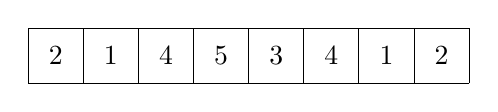
\begin{tikzpicture}[scale=0.7]
\draw (0,0) grid (8,1);

\node at (0.5,0.5) {$2$};
\node at (1.5,0.5) {$1$};
\node at (2.5,0.5) {$4$};
\node at (3.5,0.5) {$5$};
\node at (4.5,0.5) {$3$};
\node at (5.5,0.5) {$4$};
\node at (6.5,0.5) {$1$};
\node at (7.5,0.5) {$2$};
\end{tikzpicture}
\end{center}

\begin{comment}
Suppose that the size of the sliding window is 4.
At the first window position, the smallest value is 1:
\end{comment}

スライドウインドウのサイズを4としよう。
最初の位置において、最小値は1である:
\begin{center}
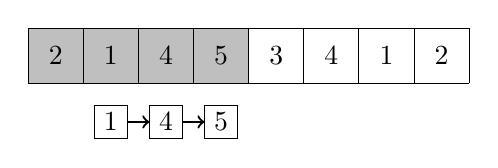
\begin{tikzpicture}[scale=0.7]
\fill[color=lightgray] (0,0) rectangle (4,1);
\draw (0,0) grid (8,1);

\node at (0.5,0.5) {$2$};
\node at (1.5,0.5) {$1$};
\node at (2.5,0.5) {$4$};
\node at (3.5,0.5) {$5$};
\node at (4.5,0.5) {$3$};
\node at (5.5,0.5) {$4$};
\node at (6.5,0.5) {$1$};
\node at (7.5,0.5) {$2$};

\draw (1.2,0.2-1.2) rectangle (1.8,0.8-1.2);
\draw (2.2,0.2-1.2) rectangle (2.8,0.8-1.2);
\draw (3.2,0.2-1.2) rectangle (3.8,0.8-1.2);

\node at (1.5,0.5-1.2) {$1$};
\node at (2.5,0.5-1.2) {$4$};
\node at (3.5,0.5-1.2) {$5$};

\draw[->,thick] (1.8,0.5-1.2) -- (2.2,0.5-1.2);
\draw[->,thick] (2.8,0.5-1.2) -- (3.2,0.5-1.2);
\end{tikzpicture}
\end{center}

\begin{comment}
Then the window moves one step right.
The new element 3 is smaller than the elements
4 and 5 in the queue, so the elements 4 and 5
are removed from the queue
and the element 3 is added to the queue.
The smallest value is still 1.
\end{comment}

ウインドウを1つ右に動かそう。
新たな要素3はすでにキューにある4,5より小さいので、
キューから4,5は取り除き、3を末尾に加える。
最小値はまだ1のままである:
\begin{center}
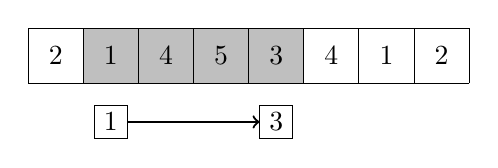
\begin{tikzpicture}[scale=0.7]
\fill[color=lightgray] (1,0) rectangle (5,1);
\draw (0,0) grid (8,1);

\node at (0.5,0.5) {$2$};
\node at (1.5,0.5) {$1$};
\node at (2.5,0.5) {$4$};
\node at (3.5,0.5) {$5$};
\node at (4.5,0.5) {$3$};
\node at (5.5,0.5) {$4$};
\node at (6.5,0.5) {$1$};
\node at (7.5,0.5) {$2$};

\draw (1.2,0.2-1.2) rectangle (1.8,0.8-1.2);
\draw (4.2,0.2-1.2) rectangle (4.8,0.8-1.2);

\node at (1.5,0.5-1.2) {$1$};
\node at (4.5,0.5-1.2) {$3$};

\draw[->,thick] (1.8,0.5-1.2) -- (4.2,0.5-1.2);
\end{tikzpicture}
\end{center}

\begin{comment}
After this, the window moves again,
and the smallest element 1
does not belong to the window anymore.
Thus, it is removed from the queue and the smallest
value is now 3. Also the new element 4
is added to the queue.
\end{comment}

その後、再度ウインドウを動かすと、
最小値1はもはやウインドウ内に無い。
よって1をキューから取り除くと、最小値は3となる。
また、新たな要素4がキューに追加される。

\begin{center}
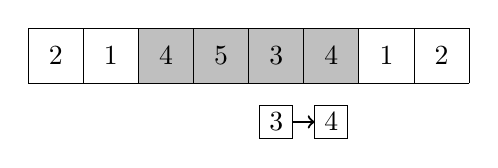
\begin{tikzpicture}[scale=0.7]
\fill[color=lightgray] (2,0) rectangle (6,1);
\draw (0,0) grid (8,1);

\node at (0.5,0.5) {$2$};
\node at (1.5,0.5) {$1$};
\node at (2.5,0.5) {$4$};
\node at (3.5,0.5) {$5$};
\node at (4.5,0.5) {$3$};
\node at (5.5,0.5) {$4$};
\node at (6.5,0.5) {$1$};
\node at (7.5,0.5) {$2$};

\draw (4.2,0.2-1.2) rectangle (4.8,0.8-1.2);
\draw (5.2,0.2-1.2) rectangle (5.8,0.8-1.2);

\node at (4.5,0.5-1.2) {$3$};
\node at (5.5,0.5-1.2) {$4$};

\draw[->,thick] (4.8,0.5-1.2) -- (5.2,0.5-1.2);
\end{tikzpicture}
\end{center}

\begin{comment}
The next new element 1 is smaller than all elements
in the queue.
Thus, all elements are removed from the queue
and it will only contain the element 1:
\end{comment}

次の新たな要素1はキューのすべての値より小さいので、
キューのすべての要素は取り除かれ、
1だけが残る:

\begin{center}
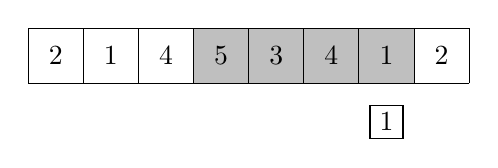
\begin{tikzpicture}[scale=0.7]
\fill[color=lightgray] (3,0) rectangle (7,1);
\draw (0,0) grid (8,1);

\node at (0.5,0.5) {$2$};
\node at (1.5,0.5) {$1$};
\node at (2.5,0.5) {$4$};
\node at (3.5,0.5) {$5$};
\node at (4.5,0.5) {$3$};
\node at (5.5,0.5) {$4$};
\node at (6.5,0.5) {$1$};
\node at (7.5,0.5) {$2$};

\draw (6.2,0.2-1.2) rectangle (6.8,0.8-1.2);

\node at (6.5,0.5-1.2) {$1$};
\end{tikzpicture}
\end{center}

\begin{comment}
Finally the window reaches its last position.
The element 2 is added to the queue,
but the smallest value inside the window
is still 1.
\end{comment}

ウインドウが終端に到達すると、
キューに要素2が追加されるが、
ウインドウ内の最小値は未だ1である。

\begin{center}
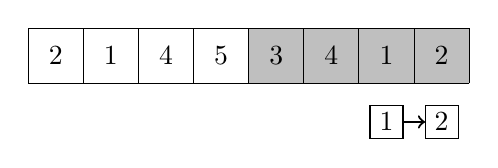
\begin{tikzpicture}[scale=0.7]
\fill[color=lightgray] (4,0) rectangle (8,1);
\draw (0,0) grid (8,1);

\node at (0.5,0.5) {$2$};
\node at (1.5,0.5) {$1$};
\node at (2.5,0.5) {$4$};
\node at (3.5,0.5) {$5$};
\node at (4.5,0.5) {$3$};
\node at (5.5,0.5) {$4$};
\node at (6.5,0.5) {$1$};
\node at (7.5,0.5) {$2$};

\draw (6.2,0.2-1.2) rectangle (6.8,0.8-1.2);
\draw (7.2,0.2-1.2) rectangle (7.8,0.8-1.2);

\node at (6.5,0.5-1.2) {$1$};
\node at (7.5,0.5-1.2) {$2$};

\draw[->,thick] (6.8,0.5-1.2) -- (7.2,0.5-1.2);
\end{tikzpicture}
\end{center}

\begin{comment}
Since each array element
is added to the queue exactly once and
removed from the queue at most once,
the algorithm works in $O(n)$ time.
\end{comment}

配列の各要素がキューに出入りするのは高々1回なので、
このアルゴリズムは$O(n)$時間で動作する。
